% XiYuan Project — Fig. 2 (revised)
% Compile with XeLaTeX:
% xelatex -interaction=nonstopmode Fig2_Unimodal_Performance_Compact_v7.tex
\documentclass[tikz,border=2.5mm]{standalone}
\usepackage{fontspec}
\usepackage{pgfplots}
\pgfplotsset{compat=1.18}
\setmainfont{Arimo}

\definecolor{ink}{HTML}{253340}
\definecolor{hair}{HTML}{BEC9D1}
\definecolor{mid}{HTML}{8999A4}
\definecolor{ir}{HTML}{3C7294}
\definecolor{ram}{HTML}{318A80}
\definecolor{uv}{HTML}{756C9D}
\definecolor{gridgray}{HTML}{DCE3E8}

\begin{document}
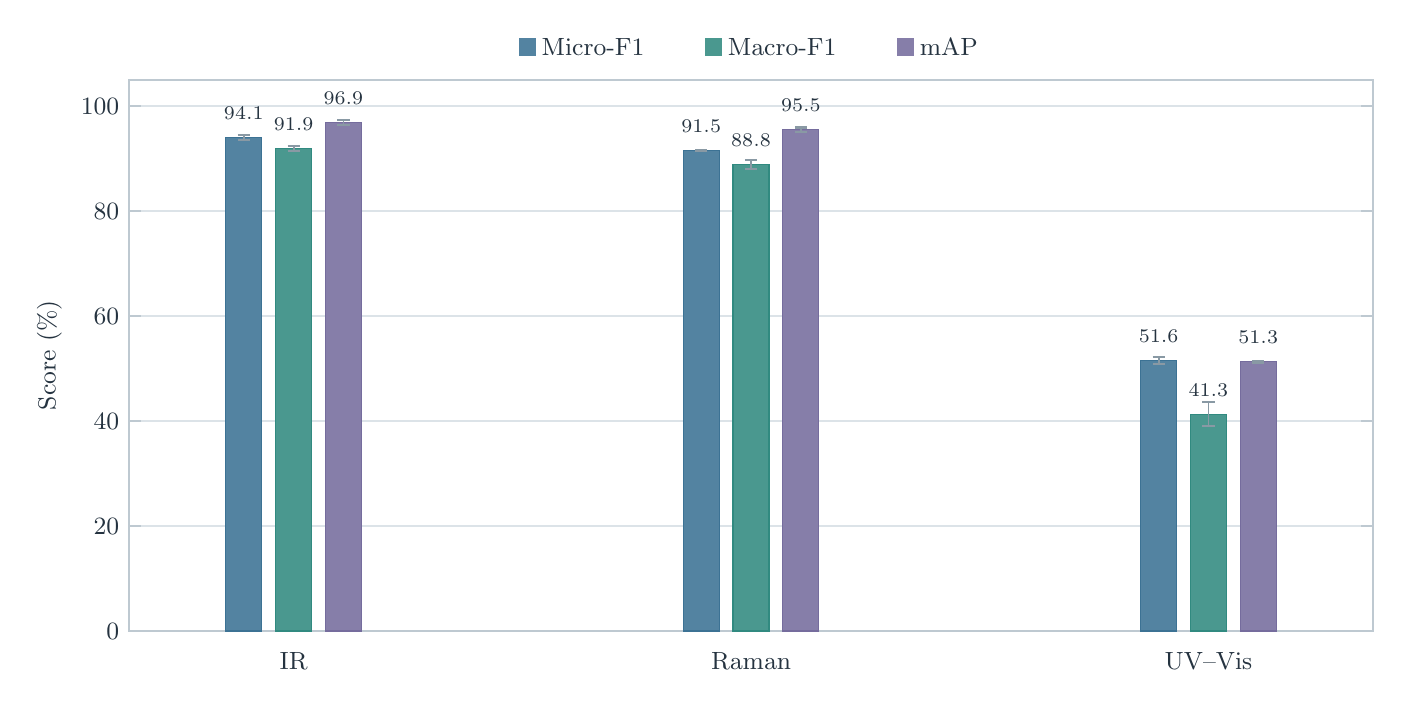
\begin{tikzpicture}
\begin{axis}[
    width=15.8cm,
    height=7.0cm,
    scale only axis,
    ymin=0, ymax=105,
    ylabel={Score (\%)},
    ylabel style={font=\small, text=ink},
    symbolic x coords={IR,Raman,UV--Vis},
    xtick=data,
    xticklabel style={font=\small, text=ink},
    ytick={0,20,40,60,80,100},
    yticklabel style={font=\small, text=ink},
    ymajorgrids=true,
    grid style={draw=gridgray,line width=0.45pt},
    axis line style={draw=hair,line width=0.7pt},
    tick style={draw=hair,line width=0.7pt},
    xtick style={draw=none},
    enlarge x limits=0.18,
    ybar=5pt,
    bar width=13pt,
    clip=false,
    legend columns=3,
    legend style={
        draw=none,
        fill=none,
        font=\small,
        text=ink,
        at={(0.5,1.015)},
        anchor=south,
        /tikz/every even column/.append style={column sep=7mm}
    },
    legend image code/.code={\draw[draw=none,fill=#1] (0cm,-0.08cm) rectangle (0.22cm,0.14cm);},
]

\addplot+[
    draw=ir, fill=ir!88,
    point meta=y,
    nodes near coords={\pgfmathprintnumber[fixed,precision=1]{\pgfplotspointmeta}},
    every node near coord/.append style={font=\scriptsize,text=ink,anchor=south,yshift=3pt},
    error bars/.cd, y dir=both, y explicit,
    error bar style={draw=mid,line width=0.65pt},
    error mark options={rotate=90,mark size=2.2pt,draw=mid,line width=0.75pt}
] coordinates {
(IR,94.0558) +- (0,0.4825)
(Raman,91.5080) +- (0,0.1382)
(UV--Vis,51.5769) +- (0,0.6746)
};
\addlegendentry{Micro-F1}

\addplot+[
    draw=ram, fill=ram!88,
    point meta=y,
    nodes near coords={\pgfmathprintnumber[fixed,precision=1]{\pgfplotspointmeta}},
    every node near coord/.append style={font=\scriptsize,text=ink,anchor=south,yshift=3pt},
    error bars/.cd, y dir=both, y explicit,
    error bar style={draw=mid,line width=0.65pt},
    error mark options={rotate=90,mark size=2.2pt,draw=mid,line width=0.75pt}
] coordinates {
(IR,91.9325) +- (0,0.4942)
(Raman,88.8480) +- (0,0.7879)
(UV--Vis,41.2964) +- (0,2.3240)
};
\addlegendentry{Macro-F1}

\addplot+[
    draw=uv, fill=uv!88,
    point meta=y,
    nodes near coords={\pgfmathprintnumber[fixed,precision=1]{\pgfplotspointmeta}},
    every node near coord/.append style={font=\scriptsize,text=ink,anchor=south,yshift=3pt},
    error bars/.cd, y dir=both, y explicit,
    error bar style={draw=mid,line width=0.65pt},
    error mark options={rotate=90,mark size=2.2pt,draw=mid,line width=0.75pt}
] coordinates {
(IR,96.8850) +- (0,0.5000)
(Raman,95.4789) +- (0,0.4389)
(UV--Vis,51.2550) +- (0,0.1074)
};
\addlegendentry{mAP}

% Numeric labels are attached to each bar coordinate, keeping exact horizontal alignment.

\end{axis}
\end{tikzpicture}
\end{document}
